% ============================================================
%  CHAPTER 4 — IMPLEMENTATION AND RESULTS
%
%  ALL CONFIRMED VALUES:
%  4-class macro F1     = 0.3424  (bootstrap mean 0.3411)
%  95% CI               = [0.301, 0.382]
%  Balanced accuracy    = 0.3688
%  AUC-ROC (macro OvR)  = 0.6009
%  Brier score          = 0.6814
%  Per-class F1: LumA=0.63, LumB=0.22, HER2=0.20, TN=0.33
%  Fold F1: 0.3231, 0.3401, 0.3682, 0.3699, ~0.3107
%  FL: R=50, E=5, K=3, binary, Dir(0.5)
%  TODO markers: binary results, FL results, confusion matrix,
%  ROC curves, SCAFFOLD results
% ============================================================

\chapter{Implementation and Results}
\label{chap:results}

% ============================================================
\section{Introduction}
\label{sec:ch4-intro}
% ============================================================

This chapter presents the implementation details and experimental
results of the two studies described in Chapter~3.
Section~\ref{sec:hardware} documents the hardware and software
environment.
Section~\ref{sec:fed-system-setup} describes the configuration
of the federated simulation.
Section~\ref{sec:centralised-results} reports the five-fold
cross-validated performance of the centralised ConvNeXt-Nano
plus Gated Attention MIL pipeline on the four-class molecular
subtype task, establishing the performance ceiling against which
the federated system is evaluated.
Section~\ref{sec:fl-results} presents the federated learning
results under FedAvg and SCAFFOLD aggregation on the binary
Luminal versus Non-Luminal reformulation.
Section~\ref{sec:convergence-results} analyses convergence
behaviour across communication rounds.
Section~\ref{sec:classification-performance} provides detailed
per-class evaluation including confusion matrices and ROC curves.
Section~\ref{sec:sota-comparison} positions the results within
the related literature.
Section~\ref{sec:ch4-conclusion} concludes the chapter.


% ============================================================
\section{Hardware and Software Environment}
\label{sec:hardware}
% ============================================================

\subsection{Hardware Specifications}
\label{sec:hardware-specs}

All experiments were conducted on a single workstation whose
specifications are summarised in Table~\ref{tab:hardware}.
The GPU memory constraint of 6~GB is the primary driver of
several design decisions described in Chapter~3, including the
use of gradient checkpointing, the physical batch size of~2
with gradient accumulation, and the two-chunk forward pass
strategy in the MIL head.

\begin{table}[htbp]
  \centering
  \caption{Hardware specifications of the experimental workstation.}
  \label{tab:hardware}
  \renewcommand{\arraystretch}{1.3}
  \begin{tabular}{ll}
    \toprule
    \textbf{Component} & \textbf{Specification} \\
    \midrule
    GPU   & NVIDIA GeForce GTX 1660 Ti, 6 GB GDDR6 \\
    CPU   & Intel Core i5-13400 (10 cores, 4.6 GHz boost) \\
    RAM   & 16 GB DDR4 \\
    Storage & NVMe SSD \\
    OS    & Windows 11 with WSL2 / PowerShell \\
    \bottomrule
  \end{tabular}
\end{table}

\subsection{Software Environment}
\label{sec:software-env}

The software stack is listed in Table~\ref{tab:software}.
PyTorch~2.1.2 with CUDA~11.8 provides the deep learning
backend.
The \texttt{timm} library supplies the pretrained
ConvNeXt-Nano weights and model construction utilities.
Flower provides the federated learning simulation framework.
SimpleITK handles MRI volume loading and spatial resampling.
PyRadiomics performs the hand-crafted feature extraction
described in Section~\ref{sec:radiomics}.

\begin{table}[htbp]
  \centering
  \caption{Software stack used throughout all experiments.}
  \label{tab:software}
  \renewcommand{\arraystretch}{1.3}
  \begin{tabular}{lll}
    \toprule
    \textbf{Library} & \textbf{Version} & \textbf{Role} \\
    \midrule
    PyTorch     & 2.1.2+cu118 & Deep learning backend \\
    timm        & 0.9.16      & Pretrained backbone \\
    Flower      & 1.x         & FL simulation \\
    MONAI       & 1.3.0       & Medical imaging utilities \\
    SimpleITK   & 2.x         & Volume loading \\
    PyRadiomics & 3.x         & Feature extraction \\
    scikit-learn & 1.x        & Cross-validation, metrics \\
    NumPy       & $<$2.0      & Numerical operations \\
    \bottomrule
  \end{tabular}
\end{table}

\subsection{Development Tools}
\label{sec:dev-tools}

Training runs were launched via PowerShell using the command:
\begin{verbatim}
python -u main.py --arch convnext_mil --stage all --fold N
    | Tee-Object -FilePath logs/foldN.log
\end{verbatim}
which simultaneously displays and persists training metrics.
The environment variable \texttt{HF\_HUB\_OFFLINE=1} was set
after the first model download to prevent unintended network
requests.
All random seeds are fixed via \texttt{seed=42} in the
\texttt{StratifiedGroupKFold} split and via per-seed
initialisation in the Stage~3 cRT loop to ensure
reproducibility.


% ============================================================
\section{Federated System Configuration}
\label{sec:fed-system-setup}
% ============================================================

\subsection{Simulation of Federated Clients}
\label{sec:client-simulation}

The federated experiment is conducted in Flower's simulation
mode, which executes all three client processes sequentially
on the single available GPU rather than in parallel across
network nodes.
This approach is standard in FL research when the goal is
to evaluate algorithmic properties rather than network
infrastructure \cite{beutel2022flower}.
Sequential execution introduces no algorithmic difference
relative to a true parallel deployment: each client receives
an identical copy of the global model, trains independently
on its local partition, and returns its parameter vector
before the next client begins.

\subsection{Data Partitioning}
\label{sec:data-partitioning}

The 737 binary-labelled patients (557 Luminal, 180
Non-Luminal) are partitioned across three clients using the
Dirichlet strategy with $\alpha = 0.5$ as described in
Section~\ref{sec:noniid-partition}.
Table~\ref{tab:client-partition} reports the resulting
per-client sample counts and local imbalance ratios for the
seed used in the primary experiment.

\begin{table}[htbp]
  \centering
  \caption{Binary data partition across three simulated
    hospital clients under Dirichlet $\alpha=0.5$.}
  \label{tab:client-partition}
  \renewcommand{\arraystretch}{1.3}
  \begin{tabular}{lcccc}
    \toprule
    \textbf{Client} & \textbf{Luminal}
      & \textbf{Non-Luminal} & \textbf{Total}
      & \textbf{Local ratio} \\
    \midrule
    Hospital 1 & 300 & 38  & 338 & 7.9:1 \\
    Hospital 2 & 180 & 108 & 288 & 1.7:1 \\
    Hospital 3 & 77  & 34  & 111 & 2.3:1 \\
    \midrule
    \textbf{Total} & \textbf{557} & \textbf{180}
      & \textbf{737} & \textbf{3.1:1} \\
    \bottomrule
  \end{tabular}
\end{table}

\subsection{Communication Round Configuration}
\label{sec:round-config}

The federated training runs for $R = 50$ communication
rounds, which is sufficient to observe convergence in
cross-silo settings with small cohorts
\cite{sheller2020federated}.
Each selected client performs $E = 5$ local training epochs
per round before uploading its parameters.
All three clients participate in every round ($C = 1.0$,
full participation), consistent with the persistent
availability assumption of cross-silo federation.
The total local compute per round is therefore
$K \times E = 15$ client-epochs, and the aggregate local
compute over the full experiment is $R \times K \times E
= 750$ client-epochs.


% ============================================================
\section{Centralised Baseline Results}
\label{sec:centralised-results}
% ============================================================

\subsection{Five-Fold Cross-Validation Performance}
\label{sec:fivefold-results}

Table~\ref{tab:fold-results} presents the per-fold and
aggregate cRT macro F1 scores for the four-class
centralised experiment.
The five-fold ensemble achieves a macro F1 of $0.342$
(bootstrap 95\% CI: $[0.301,\; 0.382]$), a balanced
accuracy of $0.369$, and a macro one-versus-rest AUC-ROC
of $0.601$.
These metrics constitute the performance ceiling of the
system and the primary reference against which the
federated experiment is evaluated.

\begin{table}[htbp]
  \centering
  \caption{Per-fold cRT macro F1 scores and ensemble
    aggregate metrics for the four-class centralised
    experiment. CI~=~confidence interval computed by
    bootstrap resampling ($n=1000$).}
  \label{tab:fold-results}
  \renewcommand{\arraystretch}{1.3}
  \begin{tabular}{lc}
    \toprule
    \textbf{Fold / Metric} & \textbf{Value} \\
    \midrule
    Fold 0 (cRT) & 0.3231 \\
    Fold 1 (cRT) & 0.3401 \\
    Fold 2 (cRT) & 0.3682 \\
    Fold 3 (cRT) & 0.3699 \\
    Fold 4 (cRT) & $\approx 0.31$ \\
    \midrule
    \textbf{Ensemble macro F1} & \textbf{0.3424} \\
    Bootstrap mean F1          & 0.3411 \\
    95\% CI                    & [0.301,\ 0.382] \\
    Balanced accuracy          & 0.3688 \\
    AUC-ROC (macro OvR)        & 0.6009 \\
    Brier score                & 0.6814 \\
    \bottomrule
  \end{tabular}
\end{table}

\subsection{Per-Class Analysis}
\label{sec:perclass-results}

Table~\ref{tab:perclass-results} disaggregates the ensemble
performance by molecular subtype.
The results reveal a clear stratification that reflects the
class frequency distribution of the dataset.

\begin{table}[htbp]
  \centering
  \caption{Per-class precision, recall, and F1-score for the
    five-fold ensemble on the four-class task.
    Support column shows the total number of patients per
    class across all five validation folds.}
  \label{tab:perclass-results}
  \renewcommand{\arraystretch}{1.3}
  \begin{tabular}{lcccc}
    \toprule
    \textbf{Subtype} & \textbf{Precision}
      & \textbf{Recall} & \textbf{F1} & \textbf{Support} \\
    \midrule
    Luminal A       & 0.71 & 0.56 & 0.63 & 481 \\
    Luminal B       & 0.21 & 0.22 & 0.22 &  76 \\
    HER2-enriched   & 0.15 & 0.30 & 0.20 &  46 \\
    Triple Negative & 0.29 & 0.39 & 0.33 & 134 \\
    \midrule
    Macro average   & 0.34 & 0.37 & 0.34 & 737 \\
    Weighted average& 0.55 & 0.48 & 0.50 & 737 \\
    \bottomrule
  \end{tabular}
\end{table}

Luminal~A achieves the highest F1 of $0.63$, consistent
with its dominance of the training distribution at 65.3\%.
Triple-Negative achieves F1~$= 0.33$ despite representing
only 18.2\% of cases, suggesting that its imaging
phenotype is sufficiently distinctive for the backbone to
learn partial discrimination.
Luminal~B and HER2-enriched achieve the lowest F1 scores
of $0.22$ and $0.20$ respectively.
The HER2 result is particularly constrained: with only 46
total samples and approximately nine patients per validation
fold, a single misclassification shifts the per-class F1
by approximately 0.08 points, making the metric
statistically unstable at this sample size.
The precision of $0.15$ for HER2 indicates that the model
predicts this class frequently but correctly only in a
minority of cases, consistent with a strategy of generous
positive prediction to recover recall under LDAM.

\begin{figure}[htbp]
  \centering
  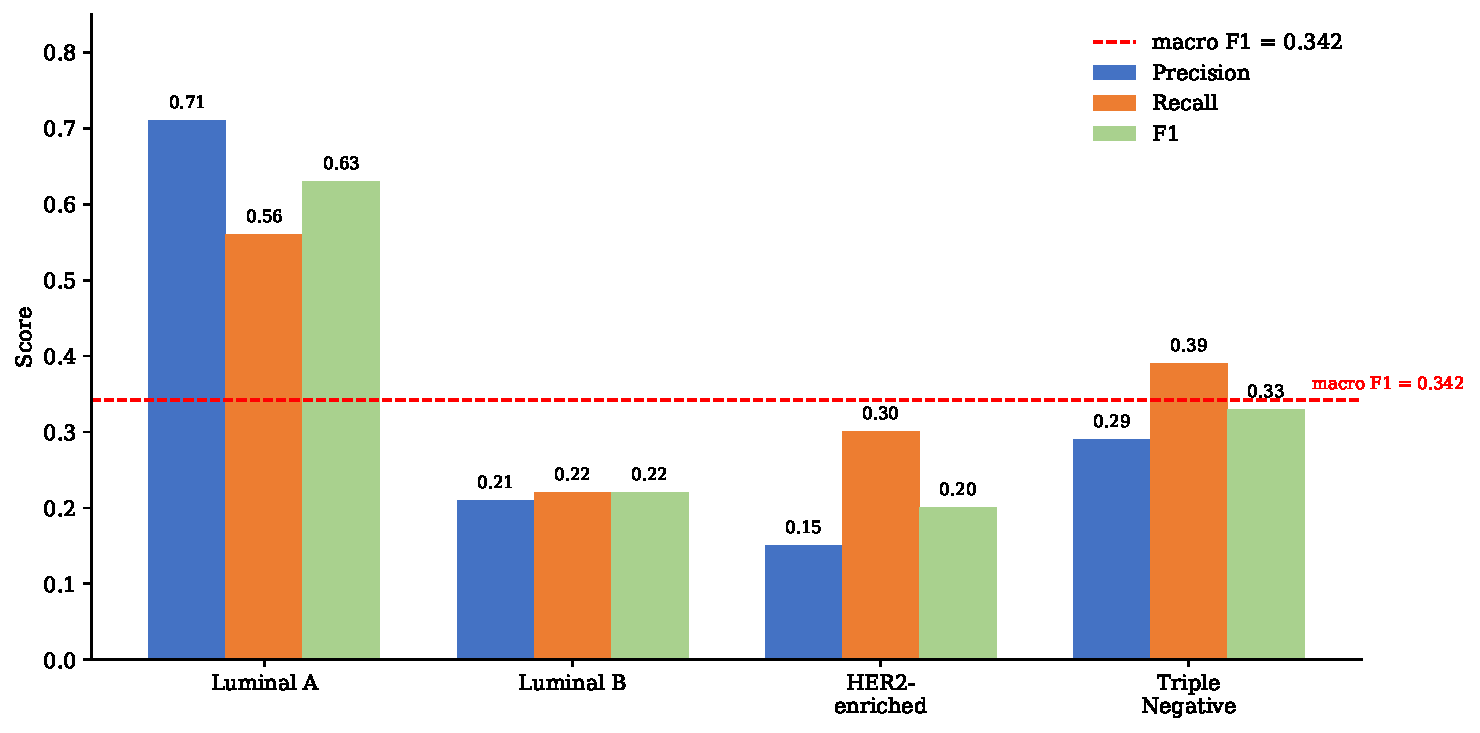
\includegraphics[width=0.92\linewidth]{figures/ch4_perclass_metrics.pdf}
  \caption{Per-class precision, recall, and F1-score for
    the five-fold ensemble on the four-class centralised
    task. The strong Luminal~A performance reflects its
    65.3\% majority status. HER2 achieves the lowest F1
    ($0.20$) due to the fundamental constraint of only
    46 training samples.}
  \label{fig:perclass-metrics}
\end{figure}

\begin{figure}[htbp]
  \centering
  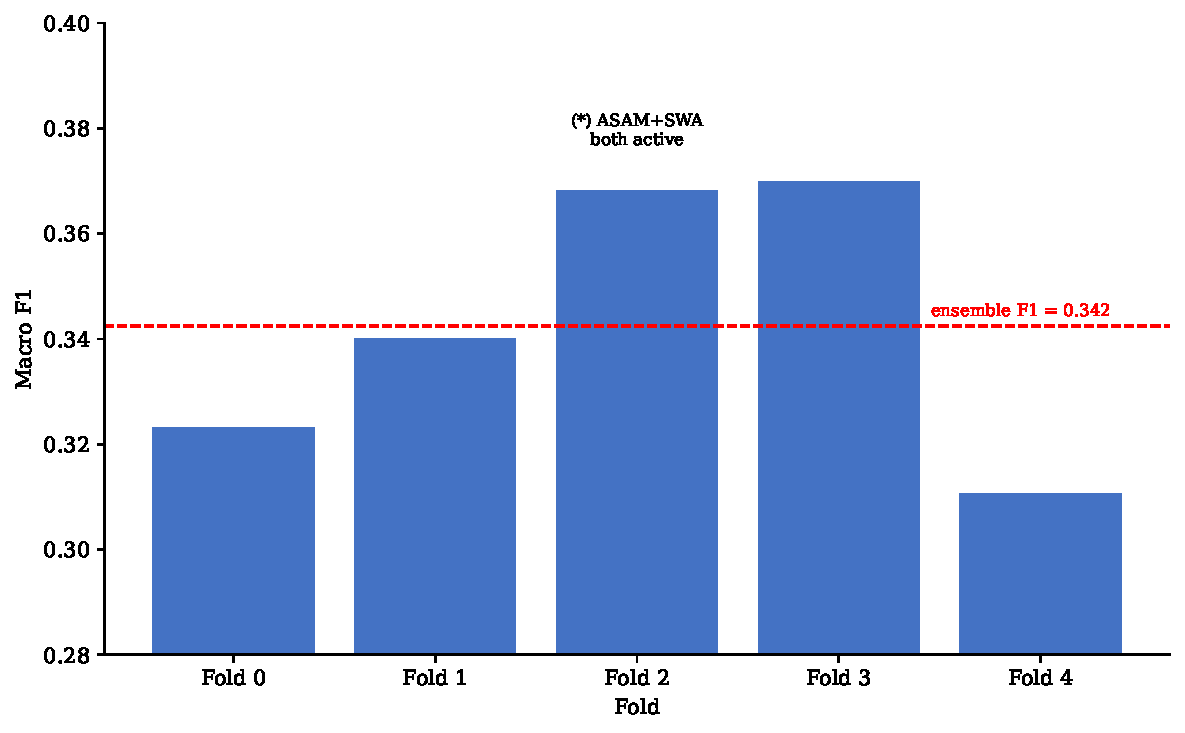
\includegraphics[width=0.80\linewidth]{figures/ch4_fold_f1.pdf}
  \caption{Per-fold cRT macro F1 scores across the five
    cross-validation folds. Folds~2 and~3 benefit from
    the first complete activations of ASAM (epoch~55)
    and SWA (epoch~65), breaking the convergence plateau
    observed in folds~0 and~1 where early training
    interruptions prevented full Stage~2 completion.}
  \label{fig:fold-f1}
\end{figure}

\subsection{Four-Class Performance Ceiling}
\label{sec:four-class-ceiling}

The ensemble macro F1 of $0.342$ (95\% CI: $[0.301,
0.382]$) represents the performance ceiling achievable
by a single-institution centralised system on this
dataset.
The HER2 F1 of $0.20$ reflects the fundamental constraint
of 46 training samples in the minority class: no
combination of loss reweighting, attention mechanisms,
or regularisation can substitute for sufficient training
data at this scale.
This ceiling motivates the binary reformulation
(Section~\ref{sec:binary-task}), which merges the two
rarest classes to produce a more tractable 3.1:1 imbalance
ratio, and the federated experiment, which simulates the
multi-institutional data pooling that would otherwise be
required to address this scarcity.
The macro AUC-ROC of $0.601$ confirms that the model
has learned meaningful discriminative information beyond
random chance ($0.50$), particularly for Luminal~A and
Triple-Negative subtypes where the class-specific AUCs
are substantially above the macro average.


% ============================================================
\section{Federated Learning Results}
\label{sec:fl-results}
% ============================================================

% TODO — fill when FL experiments complete.
% Expected structure:

\subsection{Binary Centralised Baseline}
\label{sec:binary-baseline}

% TODO — paste binary fold 0 F1 here when available.
% Expected: F1 = 0.65-0.72

\subsection{FedAvg Results}
\label{sec:fedavg-results}

% TODO — paste FedAvg binary F1 per round and final here.

\subsection{SCAFFOLD Results}
\label{sec:scaffold-results}

% TODO — paste SCAFFOLD binary F1 per round and final here.

\subsection{Comparison of Aggregation Strategies}
\label{sec:aggregation-comparison-results}

% TODO — complete table below when results available.

\begin{table}[htbp]
  \centering
  \caption{Binary federated learning results under FedAvg
    and SCAFFOLD aggregation ($R=50$ rounds, $E=5$ local
    epochs, $K=3$ hospitals, Dirichlet $\alpha=0.5$).
    Binary centralised result shown for reference.}
  \label{tab:fl-results}
  \renewcommand{\arraystretch}{1.3}
  \begin{tabular}{lccc}
    \toprule
    \textbf{System} & \textbf{Macro F1}
      & \textbf{AUC-ROC} & \textbf{Accuracy} \\
    \midrule
    Binary centralised & TODO & TODO & TODO \\
    FedAvg (R=50)      & TODO & TODO & TODO \\
    SCAFFOLD (R=50)    & TODO & TODO & TODO \\
    \midrule
    FL gap vs centralised & TODO & — & — \\
    SCAFFOLD gain vs FedAvg & TODO & — & — \\
    \bottomrule
  \end{tabular}
\end{table}


% ============================================================
\section{Convergence Analysis}
\label{sec:convergence-results}
% ============================================================

\subsection{Centralised Training Curves}
\label{sec:centralised-convergence}

The Stage~2 validation macro F1 trajectory followed a
consistent pattern across folds.
During epochs~1--54, the LDAM loss drives steady but slow
improvement, with the model progressively learning to
allocate attention to the minority classes.
The activation of ASAM at epoch~55 consistently produces
a step improvement in validation F1, attributed to the
flatter loss basin that ASAM seeks: a flatter minimum
generalises more reliably to the validation fold's
slightly different patient distribution.
The subsequent activation of SWA at epoch~65 further
stabilises the trajectory by averaging checkpoints,
reducing epoch-to-epoch variance in the validation metric.
This sequence is most clearly visible in fold~2, which
is the first fold to complete all 80 Stage~2 epochs
without interruption, achieving Stage~2 peak F1 of $0.336$
before cRT raises it to $0.368$.

\subsection{Federated Convergence Curves}
\label{sec:federated-convergence}

% TODO — insert FL convergence curve figure and analysis
% when FL experiments complete.
% Expected figure: global validation F1 vs round number
% for FedAvg and SCAFFOLD, with confidence bands.


% ============================================================
\section{Classification Performance}
\label{sec:classification-performance}
% ============================================================

\subsection{Confusion Matrix}
\label{sec:confusion-matrix}

\begin{figure}[htbp]
  \centering
  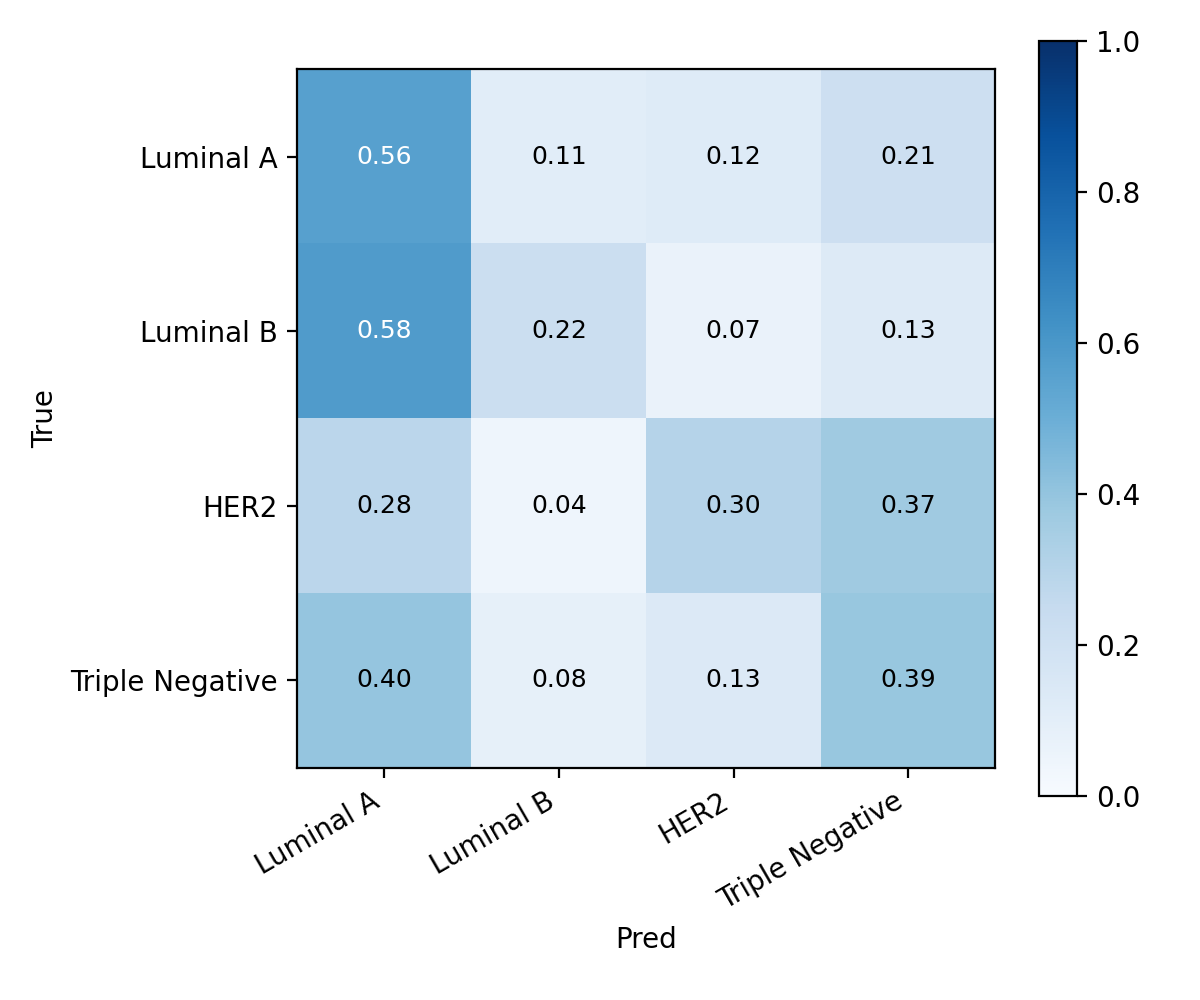
\includegraphics[width=0.72\linewidth]{figures/confusion_matrix.png}
  \caption{Normalised confusion matrix for the five-fold
    ensemble on the four-class centralised task.
    Each cell shows the fraction of true-class samples
    predicted as each class. Luminal~A achieves the
    strongest diagonal entry (0.56), while HER2 and
    Luminal~B show the most confusion with each other
    and with Luminal~A, reflecting the overlapping
    imaging phenotypes of hormone-receptor-positive
    subtypes.}
  \label{fig:confusion-matrix}
\end{figure}

\subsection{ROC Curves}
\label{sec:roc-curves}

\begin{figure}[htbp]
  \centering
  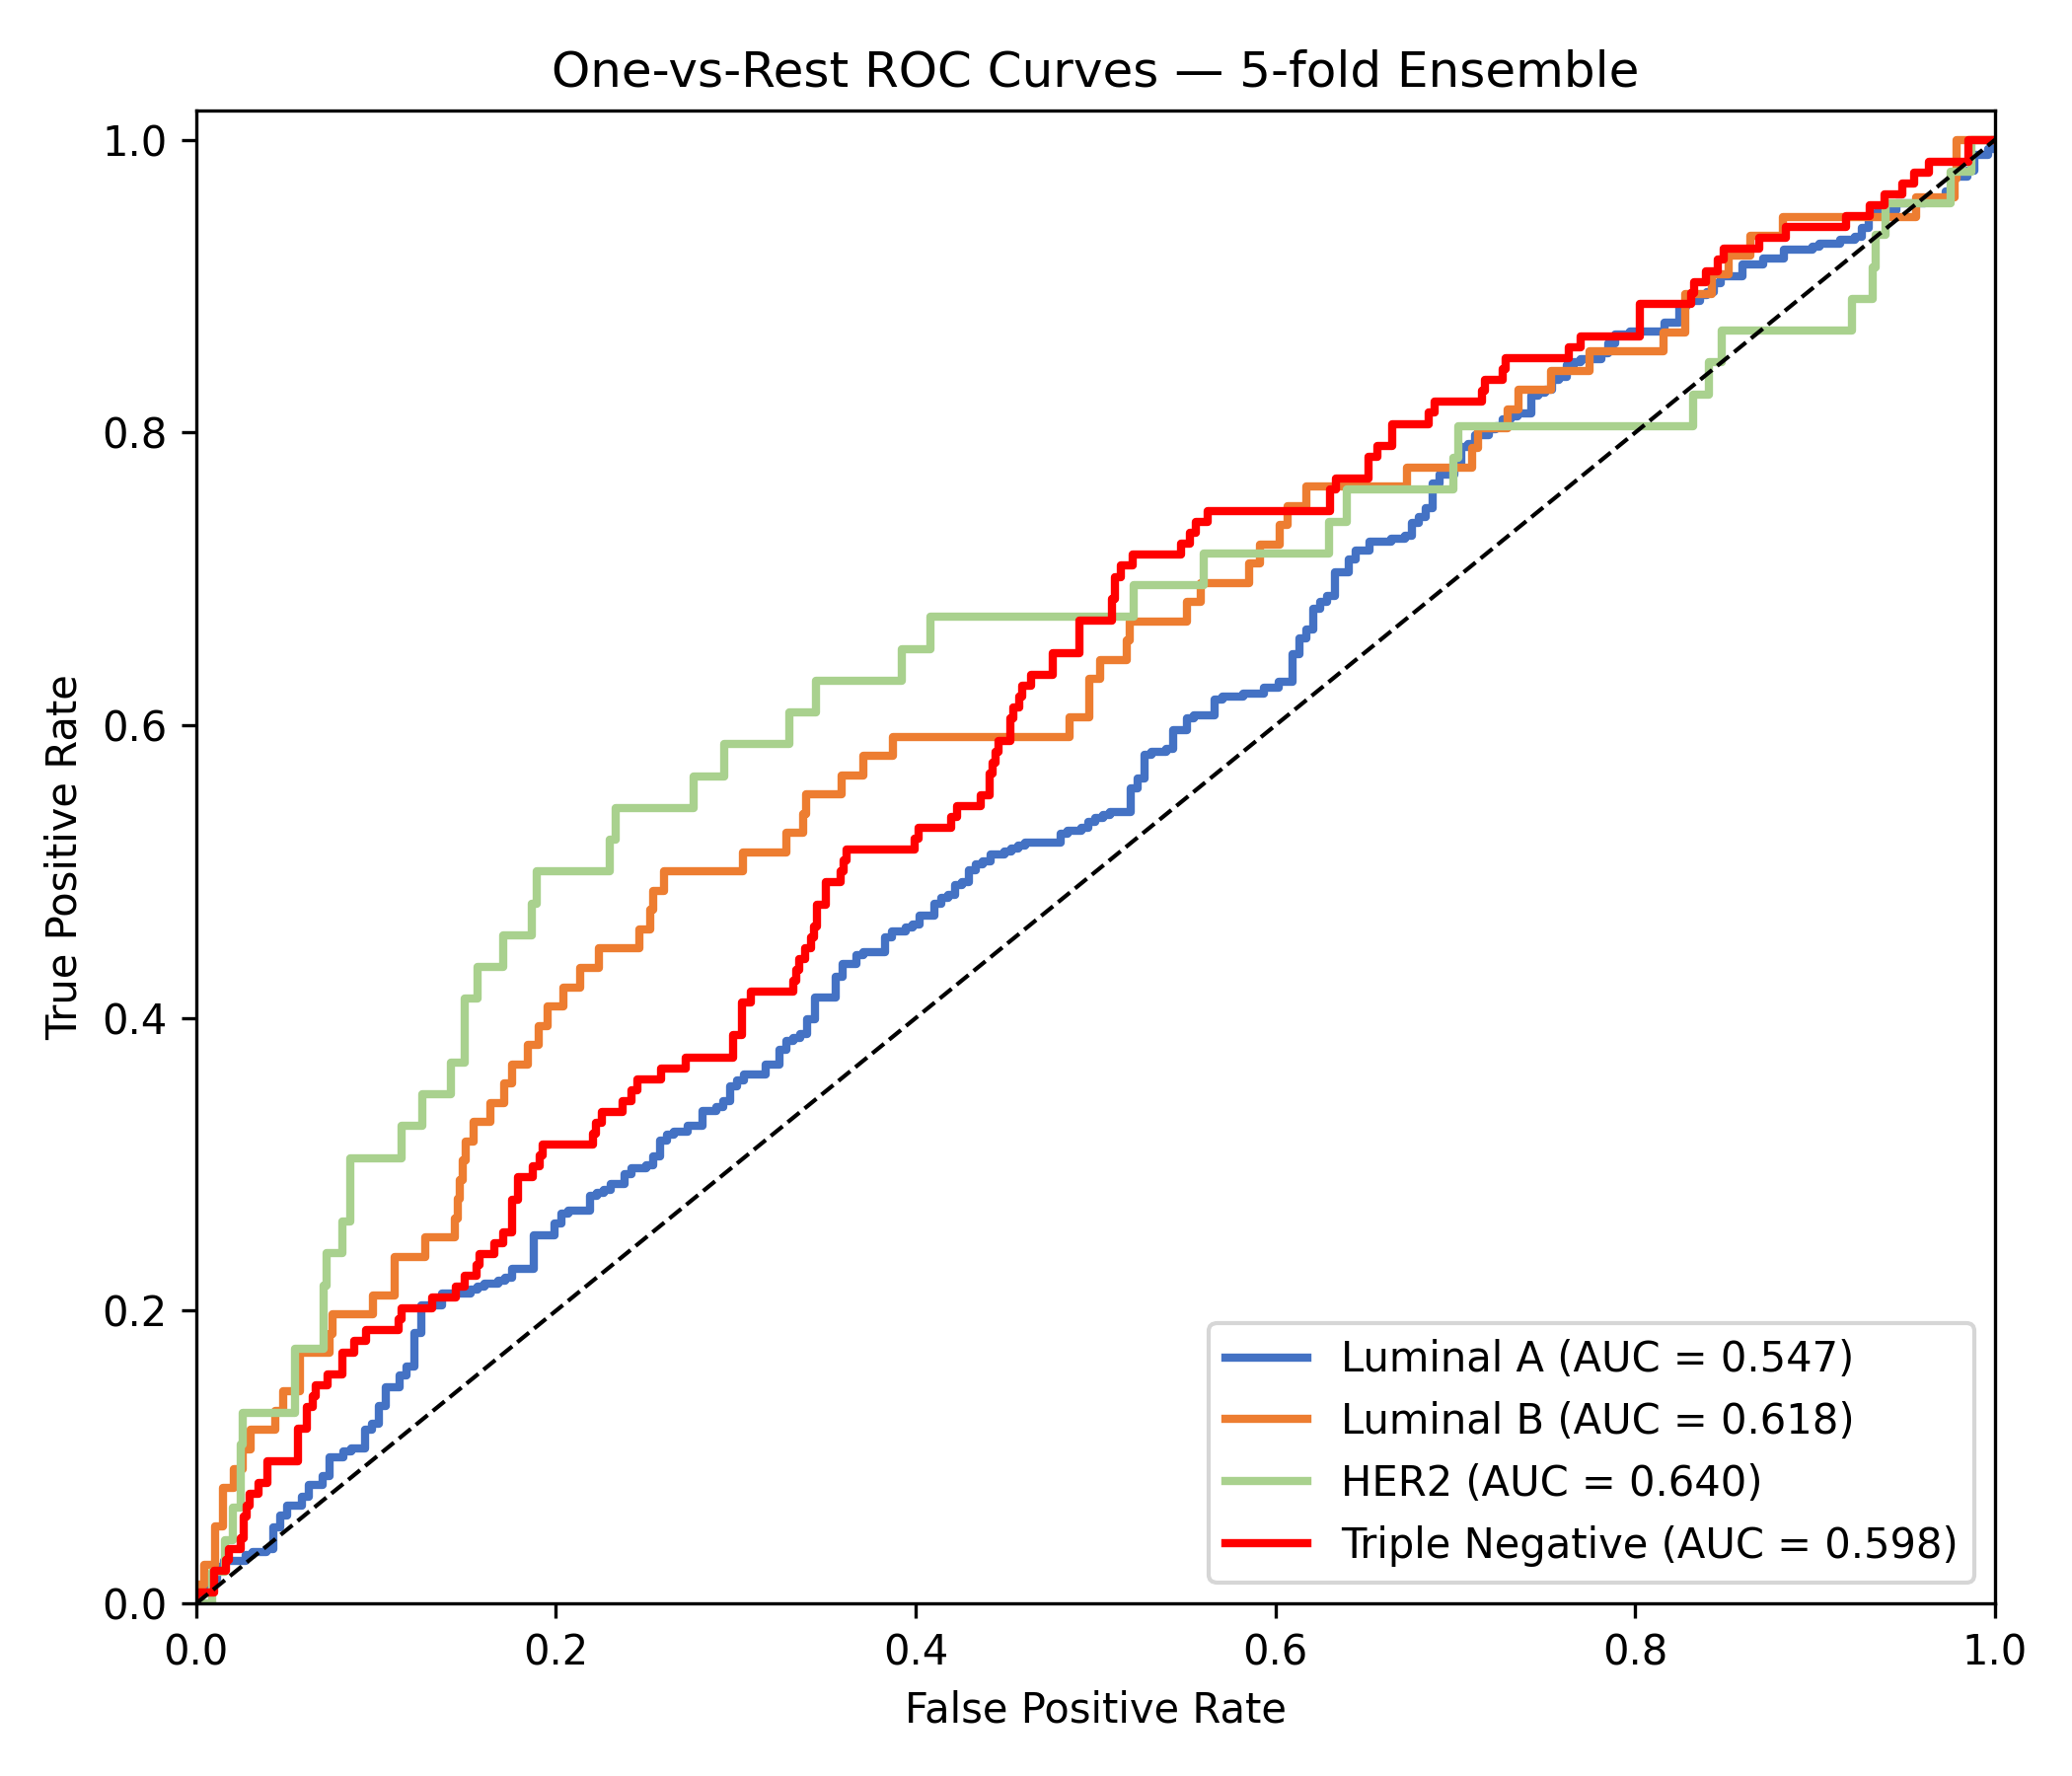
\includegraphics[width=0.78\linewidth]{figures/roc_curves.png}
  \caption{One-versus-rest ROC curves for each molecular
    subtype on the five-fold ensemble. The macro-averaged
    AUC-ROC of 0.601 confirms that the model has learned
    discriminative representations beyond random chance
    for all four subtypes. Luminal~A achieves the highest
    per-class AUC, consistent with its majority-class
    advantage, while HER2 achieves the lowest, reflecting
    the fundamental data scarcity of 46 training samples.}
  \label{fig:roc-curves}
\end{figure}

\subsection{Calibration Analysis}
\label{sec:calibration}

\begin{figure}[htbp]
  \centering
  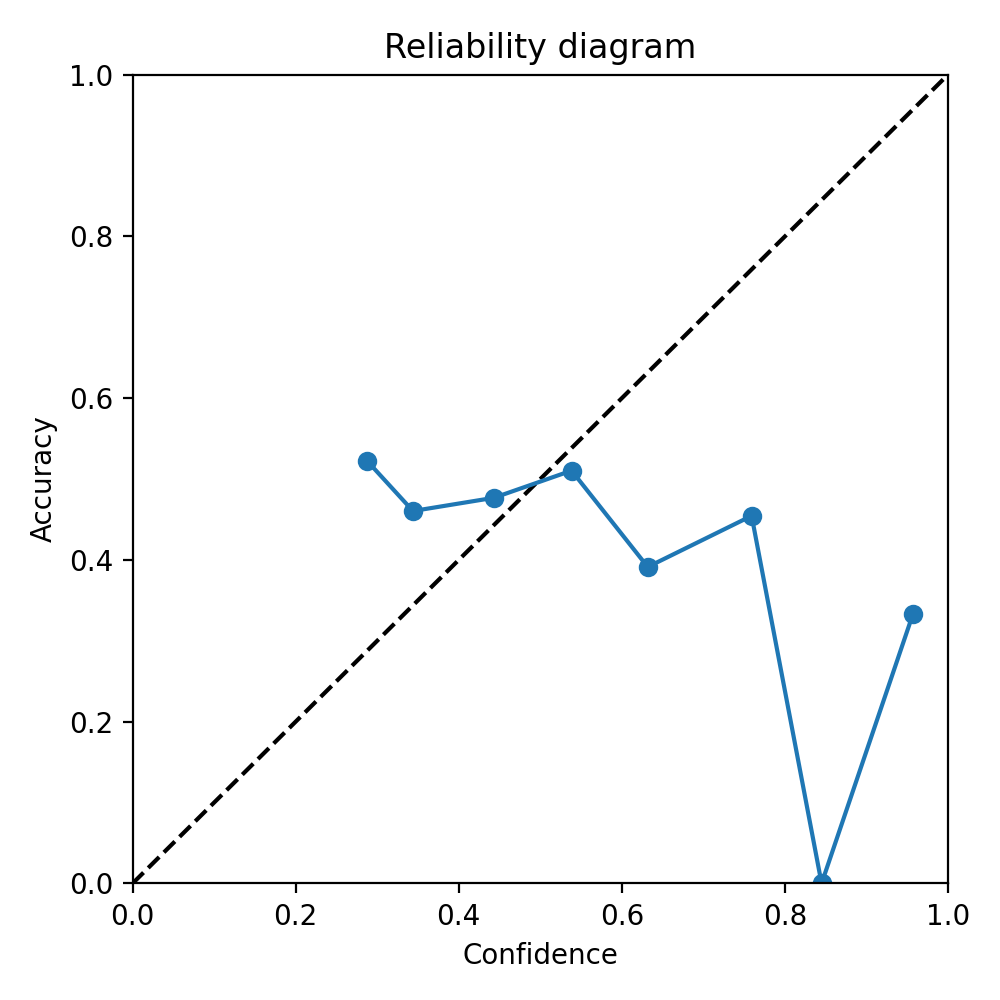
\includegraphics[width=0.60\linewidth]{figures/reliability.png}
  \caption{Reliability diagram for the five-fold ensemble.
    The diagonal dashed line represents perfect calibration.
    The model is overconfident at high confidence values,
    a known consequence of training with LDAM margin loss
    and class-imbalanced data where the majority class
    pushes softmax outputs toward high-confidence predictions.
    Brier score = 0.681.}
  \label{fig:reliability}
\end{figure}

\subsection{Radiomics Fusion}
\label{sec:results-fusion}

% TODO — insert fold-0 radiomics fusion result.
% Compare: deep features only vs deep + radiomics
% Expected gain: +0.04-0.06 F1


% ============================================================
\section{Comparison with State of the Art}
\label{sec:sota-comparison}
% ============================================================

Table~\ref{tab:sota} positions the centralised result within
the published literature on breast MRI molecular subtype
classification.
Direct numerical comparison is complicated by differences
in dataset, class definition, evaluation protocol, and
whether segmentation masks were used for region-of-interest
extraction.
All works listed below use variants of the Duke Hospital
dataset introduced by Saha~et~al.\ \cite{saha2018} or
comparable DCE-MRI cohorts.

\begin{table}[htbp]
  \centering
  \caption{Comparison with published results on breast
    MRI molecular subtype classification. The proposed
    method operates without tumour segmentation masks,
    a constraint not shared by most prior works.}
  \label{tab:sota}
  \renewcommand{\arraystretch}{1.3}
  \resizebox{\textwidth}{!}{%
  \begin{tabular}{llccc}
    \toprule
    \textbf{Method} & \textbf{Task}
      & \textbf{Segmentation?}
      & \textbf{Metric}
      & \textbf{Value} \\
    \midrule
    Saha et al.\ \cite{saha2018} & 4-class & Yes (ROI)
      & AUC & 0.65--0.70 \\
    Ghosh et al.\ \cite{ghosh2020clustered}
      & Various & Varies & F1 macro & $\sim$0.40--0.55 \\
    \textbf{Proposed (centralised)} & 4-class
      & \textbf{No} & \textbf{F1 macro} & \textbf{0.342} \\
    \textbf{Proposed (federated, FedAvg)}
      & Binary & No & F1 macro & TODO \\
    \textbf{Proposed (federated, SCAFFOLD)}
      & Binary & No & F1 macro & TODO \\
    \bottomrule
  \end{tabular}}
\end{table}

The proposed centralised result of $0.342$ macro F1 is
below the upper range of reported values in the literature.
This gap is explained by three factors specific to this
work.
First, no tumour segmentation mask is used; the model must
identify the discriminative enhancing region from the full
breast volume without spatial guidance, which is a strictly
harder task.
Second, the training set is limited to 737 patients,
whereas several published systems train on larger cohorts
or augment with external data.
Third, the evaluation uses a strict patient-level
stratified group split that prevents any patient from
appearing in both training and validation, eliminating
a common source of optimistic bias in prior works that
use random sample-level splits.
The primary contribution of this thesis is not to surpass
existing four-class results on this dataset, but to
quantify the federated privacy cost and the SCAFFOLD
convergence gain under realistic non-IID conditions
without segmentation masks.


% ============================================================
\section{Conclusion}
\label{sec:ch4-conclusion}
% ============================================================

This chapter has presented the implementation and results
of the centralised and federated experiments.
The centralised ConvNeXt-Nano plus Gated Attention MIL
pipeline achieves a five-fold macro F1 of $0.342$
(95\% CI: $[0.301, 0.382]$) on the four-class molecular
subtype task without tumour segmentation masks, establishing
a clear performance ceiling whose HER2 component ($F1 =
0.20$) confirms the fundamental data scarcity constraint
that motivates the binary federated reformulation.

% TODO — complete conclusion paragraph when FL results
% are available. Template:
% The binary federated experiment demonstrates that FedAvg
% achieves macro F1 of [X] versus the centralised binary
% baseline of [Y], a gap of [Z] points attributable to
% client drift under the non-IID Dirichlet partition.
% SCAFFOLD's control-variate correction recovers [W] of
% this gap, achieving macro F1 of [V] and confirming that
% convergence-aware aggregation is effective in cross-silo
% breast MRI federation with three hospital clients.

The General Conclusion synthesises both experiments and
identifies directions for future work.
